\documentclass{report}

\input{preamble}
\input{macros}
\input{letterfonts}

\usepackage{tikz}
\usepackage{tikz-3dplot}
\usepackage{amsmath}
\usepackage{pgfplots}
\usepackage{smartdiagram}
\usesmartdiagramlibrary{additions}

\title{\Huge{CASMA 225}\\Calc 3}
\author{\huge{Giacomo Cappelletto}}
\date{4/9/24}

\begin{document}


\maketitle
\newpage
\pdfbookmark[section]{\contentsname}{toc}
\tableofcontents
\pagebreak

\chapter{Vectors}

\section{Review}

\dfn{Notation}{

	\begin{center}
		Drawn Vectors: $\vec{v}$ \\
		Typed Vectors: \bf{v}
	\end{center}

}

\dfn{Velocity}{

	\begin{center}
		Magnitude of the velocity: $ \abs{\vec{v}} $
		\\
		Direction of the velocity: $dir(\vec{v})$
	\end{center}
}

\dfn{Heads and Tails}{

	\begin{center}
		\begin{tikzpicture}[scale=1.5]

			% Draw the vector
			\draw[->, thick] (0,0) -- (4,2) node[midway, above] {Vector $\vec{v}$};

			% Draw the tail label
			\filldraw[black] (0,0) circle (2pt);
			\node[below left] at (0,0) {Tail};

			% Draw the head label
			\filldraw[black] (4,2) circle (2pt);
			\node[above right] at (4,2) {Head};

		\end{tikzpicture}
	\end{center}
}

\nt{Scalar is like a 1 directional vector, either positive or negative, and its magnitude is the absolute value of the scalar}

\dfn{Positive y axis}{

	\begin{center}
		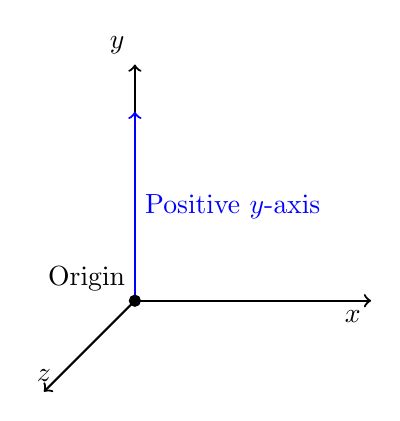
\begin{tikzpicture}[scale=2]

			% Draw the x, y, and z axes
			\draw[->, thick] (0,0,0) -- (1.5,0,0) node[anchor=north east] {$x$};
			\draw[->, thick] (0,0,0) -- (0,1.5,0) node[anchor=south east] {$y$}; % Positive y-axis
			\draw[->, thick] (0,0,0) -- (0,0,1.5) node[anchor=south] {$z$};

			% Positive y-axis with label
			\draw[->, thick, blue] (0,0,0) -- (0,1.2,0) node[midway,right] {Positive $y$-axis};

			% Draw a point at the origin
			\filldraw[black] (0,0,0) circle (1pt) node[anchor=south east] {Origin};

		\end{tikzpicture}
	\end{center}
}

\section{Vector Operations}

\dfn{Geometric POV}{
    
}

\end{document}